% Slides for TSD day

%\documentclass[usenames,dvipsnames]{beamer} % oral talk
%\documentclass[trans]{beamer}  % paper version
\mode<presentation> {
  %\usetheme{Darmstadt}
  \usetheme{Madrid}
  \usecolortheme{crane}
  %\usetheme{Goettingen}
  %\usecolortheme{wolverine}
  \setbeamercovered{transparent}
  %\useoutertheme{sidebar}
}

%Use this one for VERIMAG special barco
\setbeamercolor{frametitle}{bg=Goldenrod}
\setbeamercolor{block title}{bg=Goldenrod}


\usepackage{graphicx}
\usepackage{xspace}
\usepackage[dvips]{epsfig}
\usepackage{xmpmulti}
\usepackage{color}
\usepackage{colortbl}
\usepackage{setspace}
\usepackage{array}
\usepackage{latexsym}
\usepackage{comment}
\usepackage{amssymb,amsmath,amsthm}
\usepackage{ulem}
\usepackage{extarrows}

\usepackage {bussproofs}
\bottomAlignProof

\usepackage{dednatcol}
\usepackage{alltt}
\usepackage[latin1]{inputenc}
\usepackage{times}
\usepackage[T1]{fontenc}
\usepackage[english]{babel}

\definecolor{Blue}{rgb}{0.1,0.1,0.8}

\newcommand{\keywd}[1]{\textbf{#1}}

\setbeamercovered{dynamic}
\setbeamertemplate{theorems}[numbered]

\newcommand{\hs}{\hspace{1cm}}
\newcommand{\vs}{\vspace{1cm}}
\newcommand{\vsfive}{\vspace{5mm}}
\newcommand{\hsfive}{\hspace{5cm}}

\newcommand{\mboxfill}{\mbox{ }\hfill}

% Variables logiques

\newcommand{\rv}{\bleu {rv}\xspace}
\newcommand{\re}{\bleu {re}\xspace}
\newcommand{\rg}{\bleu {rg}\xspace}
\newcommand{\rd}{\bleu {rd}\xspace}

\newcommand{\pv}[1]{{\bleu {\textsf{I}}(\marron{#1})}}
\newcommand{\pe}[1]{{\bleu {\textsf{W}}(\marron{#1})}}
\newcommand{\pg}[1]{{\bleu {\textsf{S}}(\marron{#1})}}
\newcommand{\pd}[1]{{\bleu {\textsf{D}}(\marron{#1})}}

\newcommand{\vv}[1]{{\bleu {I}(\ensuremath{\vav{#1}})}}
\newcommand{\ve}[1]{{\bleu {W}(\ensuremath{\vav{#1}})}}
\newcommand{\vg}[1]{{\bleu {S}(\ensuremath{\vav{#1}})}}
\newcommand{\vd}[1]{{\bleu {D}(\ensuremath{\vav{#1}})}}

\newcommand{\mystrut}{\hbox to 0pt{\phantom{()}}}
%%%%%%%%%%%%%%%%%


\newtheorem{defn}{Definition}


%\newtheorem{theo}{Theorem}[section] % theorems are numbered by section
\newtheorem{theo}{Theorem} % theorems are numbered by section
\newtheorem{prop}[theo]{Proposition} % propositions are numbered as theorems
\newtheorem{lem}{Lemma} % lemmas are no longer numbered as theorems
\newtheorem{myfact}[theo]{Fact} % lemmas are numbered as theorems
\newtheorem{de}[theo]{Definition} % 

% \newcommand{\egdef}%
%    {\ensuremath{~\:\mathrel{\raisebox{-.7ex}%
%    {$\stackrel{\rm def}{=\mkern-8mu=}$}}\:~}}

\renewcommand{\impl}{\ensuremath{\Rightarrow}}


% \definecolor{marron}{rgb}{0.6, 0.2, 0}
% \definecolor{mygreen}{rgb}{0.0,0.5,0.0}
% \definecolor{brique}{rgb}{0.75, 0.05, 0}
\definecolor{violet}{rgb}{.75, 0, .75}

% \definecolor{lightblue}{rgb}{0.75,0.85,1}
% \definecolor{lightred}{rgb}{1,0.8,0.8}
% \definecolor{lightgreen}{rgb}{0.6,1,0.6}
% \definecolor{semilightgreen}{rgb}{0.5,1,0.5}
% \definecolor{lightyellow}{rgb}{1.0,1.0,0.5}
% \definecolor{lightorange}{rgb}{1.0, 0.87, 0.01}

% \newcommand{\marron}[1]{\textcolor{marron}{#1}}
% \newcommand{\brun}[1]{\textcolor{brown}{#1}}
% \newcommand{\cvert}[1]{\textcolor{mygreen}{#1}}
% \newcommand{\bleu}[1]{\textcolor{blue}{#1}}
% \newcommand{\rouge}[1]{\textcolor{red}{#1}}
% \newcommand{\brique}[1]{\textcolor{brique}{#1}}
% \newcommand{\violet}[1]{\textcolor{violet}{#1}}

\newcommand{\cdat}{\violet}
\newcommand{\cloc}{\cvert}

% ----------------------------------------------------------------------
\newcommand{\loc}{\cloc{\textit{loc}}}
\newcommand{\lx}{\cloc{\textit{x}}}
\newcommand{\ly}{\cloc{\textit{y}}}

\newcommand{\edge}[2]{\ensuremath{\cloc{#1\!\mathbin{\rightarrow}\! #2}}}
\newcommand{\cdb}{\ensuremath{\mathcal{\cdat C}}}
\newcommand{\incdb}[1]{\ensuremath{#1\in\cdb}}
\newcommand{\nincdb}[1]{\ensuremath{#1\not\in\cdb}}
\newcommand{\cdbp}{\ensuremath{\cdat{\mathcal{C}'}}}
\newcommand{\incdbp}[1]{\ensuremath{#1\in\cdbp}}
\newcommand{\nincdbp}[1]{\ensuremath{#1\not\in\cdbp}}
\newcommand{\atloc}[1]{\cdat{\ensuremath{\left|\cloc{#1}\right|}}}
\newcommand{\inset}[2]{\ensuremath{#1\in#2}}
\newcommand{\inloc}[2]{\ensuremath{#1\in\atloc{#2}}}
\newcommand{\ninloc}[2]{\ensuremath{#1\not\in\atloc{#2}}}
\newcommand{\visloc}[2]{\ensuremath{#1\in\cdat{\overline{\atloc{#2}}}}}
\newcommand{\nvisloc}[2]{\ensuremath{#1\not\in\cdat{\overline{\atloc{#2}}}}}
\newcommand{\inedge}[3]{\inloc{#1}{\edge{#2}{#3}}}
\newcommand{\ninedge}[3]{\ninloc{#1}{\edge{#2}{#3}}}
\newcommand{\cnf}{\textit{\cdat{cnf}}}
\newcommand{\pre}{\cdat{\textit{pre}}}
\newcommand{\post}{\cdat{\textit{post}}}
\newcommand{\extconfpar}[2]{\cdat{\ensuremath{\langle #1, #2\rangle}}}
\newcommand{\extconf}{\extconfpar{\cnf}{\cdb}}
\newcommand{\extconfpre}{\extconfpar{\pre}{\cdb}}
\newcommand{\extconfpost}{\extconfpar{\post}{\cdbp}}
%\newcommand{\entails}{~\rhd~}
\newcommand{\entailstrans}{\:\xrightarrow{\:trans\:}\:} % general
\newcommand{\entailsp}{\:\xrightarrow{\:sr\:}\:} % pure synchronous round
\newcommand{\entailso}{\:\xrightarrow{\:or\:}\:} % oracle round
\newcommand{\entails}{\:\xrightarrow{\:sor\:}\:} % synchronous + oracle round
\newcommand{\roas}{\textsc{roas}}
\newcommand{\roasat}[2]{\ensuremath{\roas\,@\,\edge{#1}{#2}}}
\newcommand{\roasto}[1]{\ensuremath{\roas\,@\,\cloc{\overline{#1}}}}
\newcommand{\goodat}[2]{\ensuremath{good\,@\,\edge{#1}{#2}}}
\newcommand{\goodto}[1]{\ensuremath{good\,@\,\cloc{\overline{#1}}}}
\newcommand{\correctonSTat}[1]{\ensuremath{\mbox{correct-onST}\,@\,\cloc{#1}}}
\newcommand{\wcorrectonSTat}[1]{\ensuremath{\mbox{weak-correct-onST}\,@\,\cloc{#1}}}
\newcommand{\completeonSTat}[1]{\ensuremath{\mbox{complete-onST}\,@\,\cloc{#1}}}
\newcommand{\readyat}[1]{\ensuremath{\mbox{ready}\,@\,\cloc{#1}}}
\newcommand{\correctSTat}[1]{\ensuremath{\mbox{correct-ST}\,@\,\cloc{#1}}}
\newcommand{\completeSTat}[1]{\ensuremath{\mbox{complete-ST}\,@\,\cloc{#1}}}
\newcommand{\invarat}[1]{\ensuremath{\mbox{invar}\,@\,\cloc{#1}}}


\newcommand{\hcinv}{\texttt{hc\_inversion}\xspace}

\newcommand<>{\onlybleu}[1]{{\color#2{blue}#1}}
\newcommand<>{\onlybrique}[1]{{\color#2{brique}#1}}
\newcommand<>{\onlyviolet}[1]{{\color#2{violet}#1}}


% Front page

\title[Handcrafted Small Inversions]{Handcrafted Small Inversions Made Operational on Operational Semantics}

%\subtitle{No subtitle}
\bigskip
\author[JF. Monin, X. Shi] % (optional, nur bei vielen Autoren)
{\large Jean-Fran\c{c}ois Monin \& Xiaomu Shi \\[1ex] 
  \small LIAMA Beijing, VERIMAG Grenoble}

\institute[LIAMA, VERIMAG]

\date[July 26th, 2013]

\begin{document}

\frame{\titlepage

\vfill

}

\section<presentation>*{Outline}

\begin{frame}
  \frametitle{Outline}
  %\setcounter{tocdepth}{2}
  \tableofcontents[subsectionstyle=hide]%[part=1,pausesections]
\end{frame}

% \AtBeginSubsection[] {
%   \begin{frame}<handout>
%     \frametitle{Outline}
%     \tableofcontents[sectionstyle=hide,currentsubsection]
%   \end{frame}
% }

\AtBeginSection[] {
  \begin{frame}<beamer>
    \frametitle{Outline}
    \setcounter{tocdepth}{2}
    \tableofcontents[current,subsection]
  \end{frame}
}


%%%%%%%%%%%%%%%%%%%%%%%%%%%%%%%%%%%%%%%%%%%%%%%%%%%
%%%%%%%%%%%%%%%%%%%%%%%%%%%%%%%%%%%%%%%%%%%%%%%%%%%
\section{Motivation}

\begin{frame}
\frametitle{Inversion}

\begin{block}{Forward reasoning step of choice}

Given a goal containing an hypothesis $H:P$

such that $P$ is (co)inductively defined

extract all useful information from $H$ in the environment

\end{block}

\vfill

\begin{block}{Special case of Case Analysis}

But a subtle one : na�ve use of \texttt{case} or \texttt{destruct} fails

\end{block}

\end{frame}


\begin{frame}[fragile]
\frametitle{Simple example}
\small
\begin{alltt}
\brique{
Inductive te : Type :=
  | te_const : nat -> te
  | te_plus : te -> te -> te
  | te_div0 : te -> te.}

Inductive val : Type :=
  | nval  : nat -> val
  | bval  : bool -> val.

Inductive eval : te -> val -> Prop :=
  | E_Const : forall n,
      eval (\brique{te_const} n) (nval n)
  | E_Plus : forall t1 t2 n1 n2,
      eval t1 (nval n1) ->
      eval t2 (nval n2) ->
      eval (\brique{te_plus} t1 t2) (nval (plus n1 n2)).
\end{alltt}
\end{frame}

\begin{frame}[fragile]
\frametitle{Coq built-in inversion (Cornes \& Terrasse, 1995)}
\small
\begin{alltt}
Inductive eval : te -> val -> Prop :=
  | E_Const : forall n,
      \bleu{eval} (\brique{te_const} n) (nval n)
  | E_Plus : forall t1 t2 n1 n2,
      eval t1 (nval n1) ->
      eval t2 (nval n2) ->
      \bleu{eval} (\brique{te_plus} t1 t2) (nval (plus n1 n2)).
\end{alltt}
Consider the goal:

\begin{alltt}
e : \bleu{eval} (\brique{\textbf{te_div0}} (\brique{te_const} 1)) v
============================
3 = 5
\end{alltt}
\pause %
Using Coq built-in inversion:
\begin{alltt}
\textbf{inversion} e.
\end{alltt}

\vfill

\end{frame}

\begin{frame}[fragile]
\frametitle{Coq built-in inversion (Cornes \& Terrasse, 1995)}
\small
\begin{alltt}
Inductive eval : te -> val -> Prop :=
  | E_Const : forall n,
      \bleu{eval} (\brique{te_const} n) (nval n)
  | E_Plus : forall t1 t2 n1 n2,
      eval t1 (nval n1) ->
      eval t2 (nval n2) ->
      \bleu{eval} (\brique{\textbf{te_plus}} t1 t2) (nval (plus n1 n2)).
\end{alltt}
Consider the goal:

\begin{alltt}
e : \bleu{eval} (\brique{\textbf{te_plus}} (\brique{te_const} 1) (\brique{te_const} 2)) v
============================
v = nval 3
\end{alltt}

\mbox{}
\begin{alltt}
\mbox{}
\end{alltt}

\vfill

\end{frame}


\begin{frame}[fragile]
\frametitle{Coq built-in inversion (Cornes \& Terrasse, 1995)}
\small
\begin{alltt}
e : \bleu{eval} (\brique{\textbf{te_plus}} (\brique{te_const} 1) (\brique{te_const} 2)) v
============================
v = nval 3
\end{alltt}
Using Coq built-in inversion:
\begin{alltt}
\textbf{inversion} e; subst.
...
\brique{H1} : eval (\brique{te_const} 1) (nval n1)
\brique{H3} : eval (\brique{te_const} 2) (nval n2)
============================
nval (n1 + n2) = nval 3
\end{alltt}
\end{frame}

\begin{frame}[fragile]
\hfil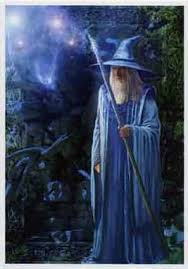
\includegraphics[width=.6\linewidth]{fig/merlin.jpg}
\end{frame}

\begin{frame}[fragile]
\frametitle{Issue when using CompCert C semantics}
\small
\begin{alltt}
H:eval_expr (Genv.globalenv prog_adc) e m RV
   (\brique{Ecall} (\brique{Evalof} (\brique{Evar} copy_StatusRegister T14) T14)
      (\brique{Econs}
         (\brique{Eaddrof}
            (\brique{Efield} (\brique{Ederef} (\brique{Evalof} (\brique{Evar} proc T3) T3) T6)
              adc_compcert.cpsr T7) T8)
         (\brique{Econs}
            (\brique{Ecall} (\brique{Evalof} (\brique{Evar} spsr T15) T15)
               (\brique{Econs} (\brique{Evalof} (\brique{Evar} proc T3) T3) \brique{Enil}) T8)
                \brique{Enil}))
      T12) t m' a'
============================
   proc_state_related m' e st'
\end{alltt}
\begin{alltt}
\bleu{
  inv H. inv H4. inv H9. inv H5. inv H4. inv H5. 
  inv H15. inv H4. inv H5. inv H14. inv H4. inv H3. 
  inv H15. inv H5. inv H4. inv H5. inv H21. inv H13.
  ...}
\end{alltt}
\end{frame}
\begin{frame}


\frametitle{Summary on built-in inversion}

\begin{block}{Nice features}
\begin{itemize}
\item Automatic
\item Works in most practical cases
\end{itemize}
  
\end{block}

\begin{block}{Drawbacks}

\begin{itemize}
\item Basic version: no control on generated names, \\
  scripts are \brique{unmanageable} during maintenance.
\item
  Controlled version \texttt{inversion...as...} : \\
  have to manually give \brique{a lot of names}.
\item
The underlying proof term is complicated \\ 
$\fl$ \brique{time consuming} when designing the script.
\item
Especially harmful with large inductive types, e.g. from Compcert
\end{itemize}
  
\end{block}

\end{frame}

%%%%%%%%%%%%%%%%%%%%%%%%%%%%%%%%%%%%%%%%%%%%%%%%%%%

\section{Absurd Cases}

\begin{frame}[fragile]
\frametitle{Absurd Cases (Small Inversions, 2010)}

\begin{alltt}
e : \bleu{eval} \brique{(te_div0 (te_const 1))} v
============================
3 = 5


  pose (\textbf{diag} t :=
  match t with
    | \brique{te_div0 (te_const 1)} => \cvert{3 = 5}
    | _ => True
  end).
  change (\textbf{diag} \brique{(te_div0 (te_const 1))}).
  destruct e; simpl; exact I.
\end{alltt}

\end{frame}



\begin{frame}
\frametitle{Small Inversions, 2010}

\begin{itemize}
\item Depends on 
  \begin{itemize}
  \item the hypothesis to be inverted (OK)
  \item the conclusion (questionable)\\
    unconvenient for massive usage
  \end{itemize}

\bigskip

\item Issues when considering relevant cases 
  \begin{itemize}
  \item additional interactions
  \item not satisfactory for inversions leading to further interactions
  \end{itemize}

\bigskip

\item But the approach is very flexible

\end{itemize}

\end{frame}



\begin{frame}[fragile]
\frametitle{A more modular variant}


\begin{alltt}
Definition inv_eval_1_div0 {t} {v} (e: eval t v) :=
  let \textbf{diag} \brique{t} :=
  match \brique{t} with
    | \brique{te_div0} n => \cvert{\(\forall\) X: Prop, X}
    | _ => True
  end
  in match e in eval \brique{t} v return \textbf{diag} \brique{t} with
       | E_Const n => I
       | E_Plus _ _ n1 n2 H1 H2 => I
  end.

e : \bleu{eval} (\brique{te_div0} (te_const 1)) v
============================
\cvert{3 = 5}

  apply (inv_eval_1_div0 e).
\end{alltt}

\end{frame}




%%%%%%%%%%%%%%%%%%%%%%%%%%%%%%%%%%%%%%%%%%%%%%%%%%%

\section{Relevant Cases}



\begin{frame}<handout:3>[fragile]
\frametitle{The diagonalization function}
\begin{itemize}
\item<1-> \cvert{yields the premises of focused constructor}
\item<2-> \bleu{independent from specific conclusion}
\item<3-> \violet{takes bindings into account}
%\item
\end{itemize}
For constructor \texttt{E\_Plus}:
\begin{semiverbatim}
\textbf{diag} t v := match t with
  | \brique{te_plus} tc1 tc2 =>
      \onlybleu<2->{\(\forall\) X: te -> Prop,}
        (\cvert{\(\forall\) n1 n2, eval tc1 (nval n1) ->
                  eval tc2 (nval n2)} -> 
                  \onlybleu<2->{X} \onlyviolet<3->{(nval (plus n1 n2))}) -> \onlybleu<2->{X} \onlyviolet<3->{v}
  | _ => True
end
\end{semiverbatim}
\end{frame}


\begin{frame}[fragile]
\frametitle{Inversion function for  ~\texttt{E\_plus}}
%\frametitle{The dedicated Ltac definition}
\small
\begin{alltt}
Definition \textbf{inv_plus_1} \{t\} \{v\} (e: eval t v) :=
  match e in (eval t v) return \textbf{diag} t v with
    | \bleu{E_Plus} _ _ n1 n2 e1 e2 => (fun X k => k n1 n2 e1 e2)
    | _ => I
  end.
\end{alltt}

\medskip
Usage:
\begin{alltt}
e : \bleu{eval} (\brique{te_plus} (\brique{te_const} 1) (\brique{te_const} 2)) v
============================
v = nval 3

apply (\textbf{inv_plus_1} e); intros \cvert{n1 n2 e1 e2}.

\cvert{e1} : eval (\brique{te_const} 1) (nval \cvert{n1})
\cvert{e2} : eval (\brique{te_const} 2) (nval \cvert{n2})
============================
nval (\cvert{n1} + \cvert{n2}) = nval 3
\end{alltt}
\end{frame}

\begin{frame}
\frametitle{More on inversion functions}

Variant are possible, e.g. \\
merging inversion functions dedicated to all constructors

\vfill

Different variants are needed in different situations

\vfill

\bleu{See demo}
\end{frame}

\begin{frame}[fragile,fragile]
\frametitle{Handcrafted inversion may beat standard inversion}

\begin{alltt}
Inductive t : nat -> Set :=
    | \brique{F1} : \(\forall\) \{n\}, t (S n)
    | \brique{FS} : \(\forall\) \{n\}, t n -> t (S n).

Inductive odd : \(\forall\) n : nat, t n -> Prop :=
   | \bleu{odd_1} : \(\forall\) n, odd (S n) \brique{F1}
   | \bleu{odd_SS} : \(\forall\) n i, odd n i -> odd _ (\brique{FS} (\brique{FS} i)).
\end{alltt}

\end{frame}

%%%%%%%%%%%%%%%%%%%%%%%%%%%%%%%%%%%%%%%%%%%%%%%%%%%

\section{Application}

\begin{frame}<1-|handout:O>
\frametitle{SimSoC: a simulator of systems-on-chip}
\hfil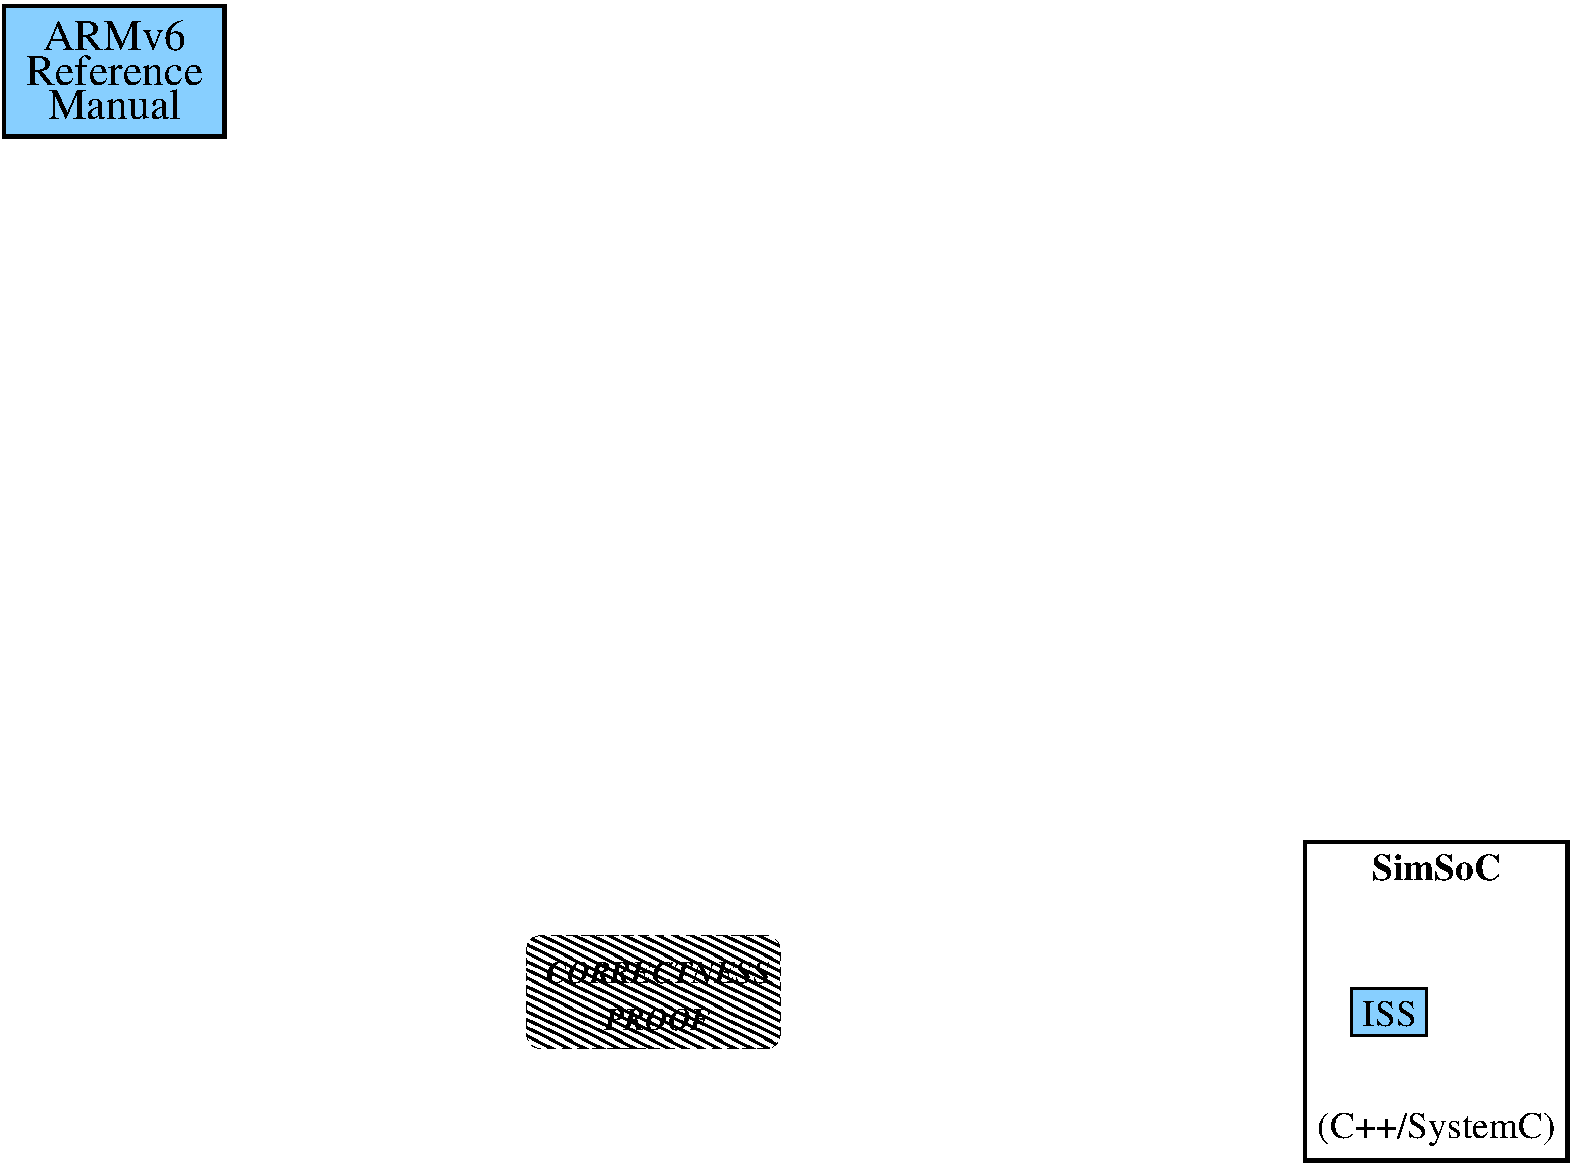
\includegraphics[width=.9\linewidth]{fig/maingen.pdf}
\end{frame}

\begin{frame}
\frametitle{SimSoC: a simulator of systems-on-chip}
\hfil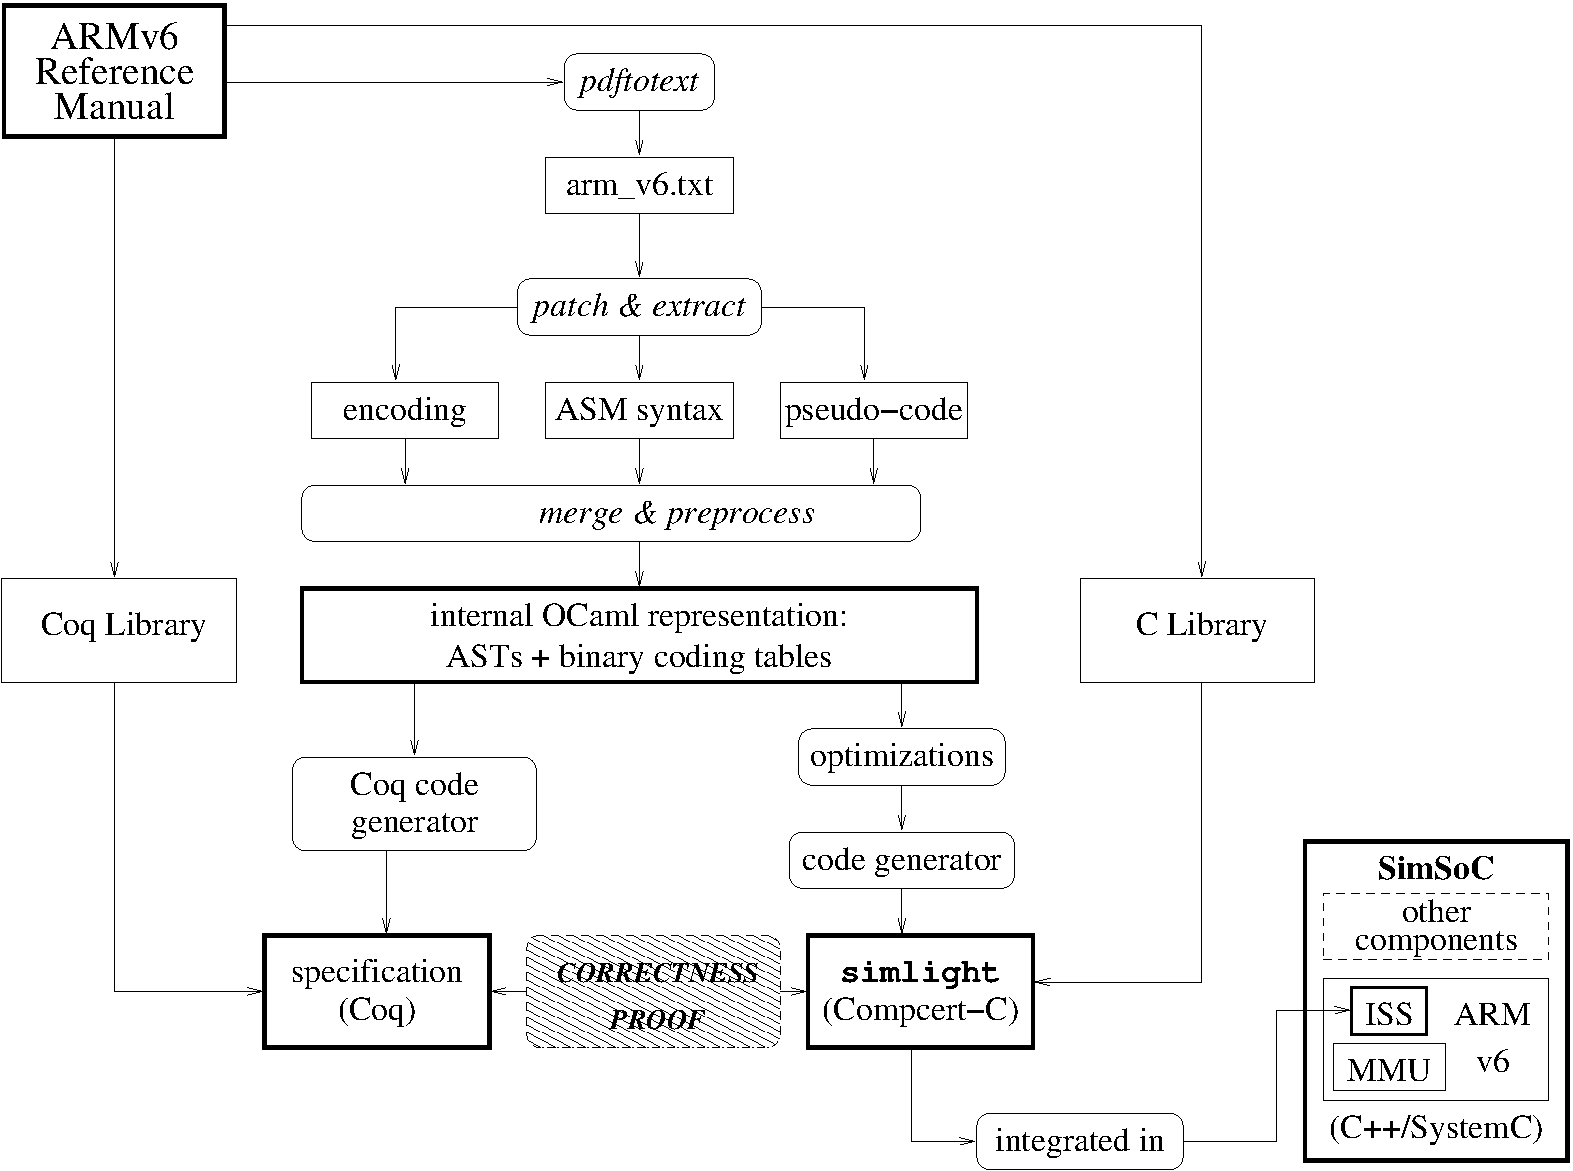
\includegraphics[width=.9\linewidth]{fig/fullarchi.pdf}
\end{frame}

\begin{frame}<1-|handout:O>
\frametitle{Projection of ARMv6 processor state ~~(excerpt)}
\hfil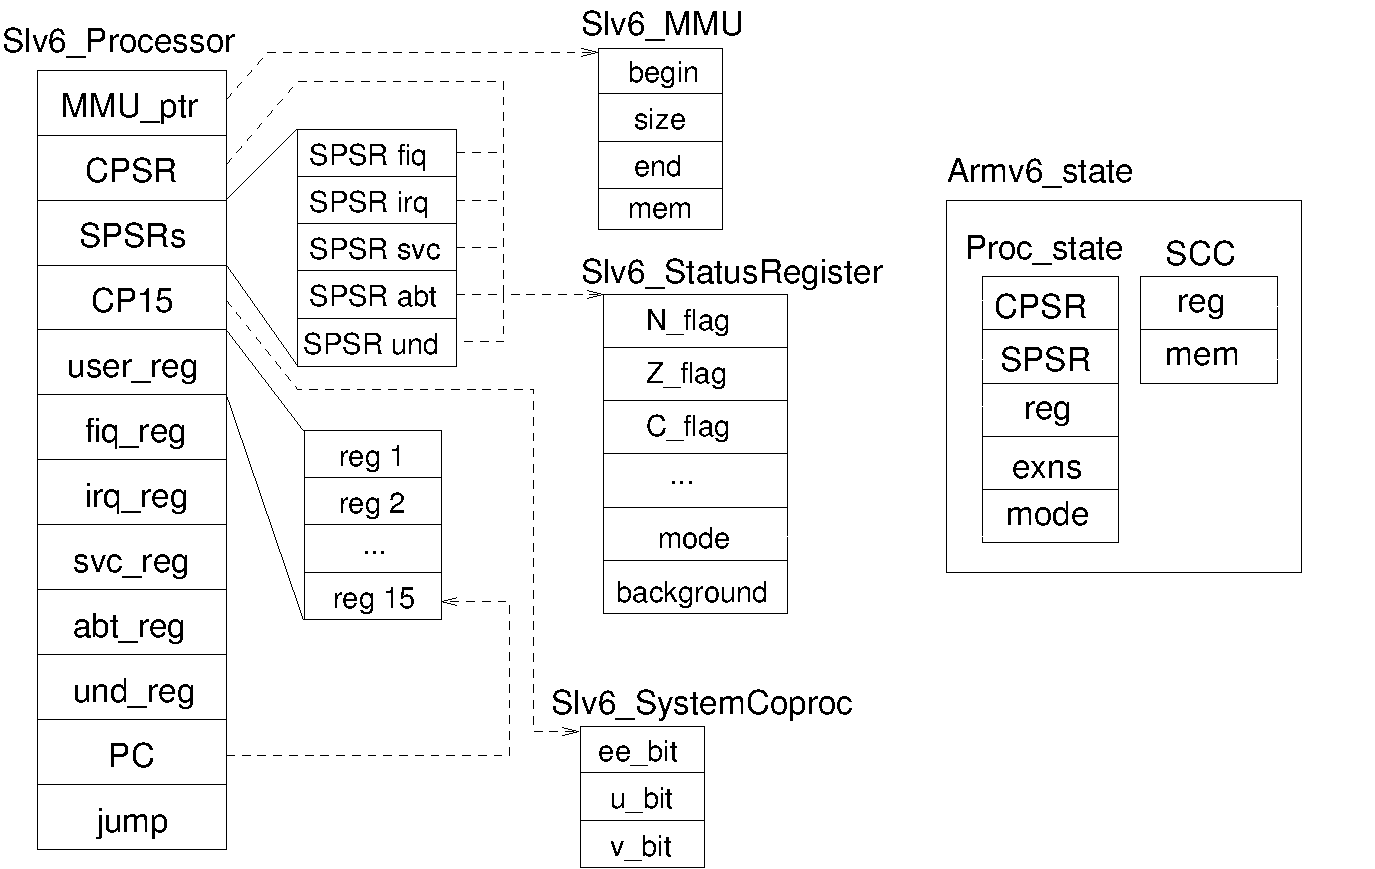
\includegraphics[width=1.01\linewidth]{fig/projection1.pdf}
\end{frame}

\begin{frame}
\frametitle{Projection of ARMv6 processor state ~~(excerpt)}
\hfil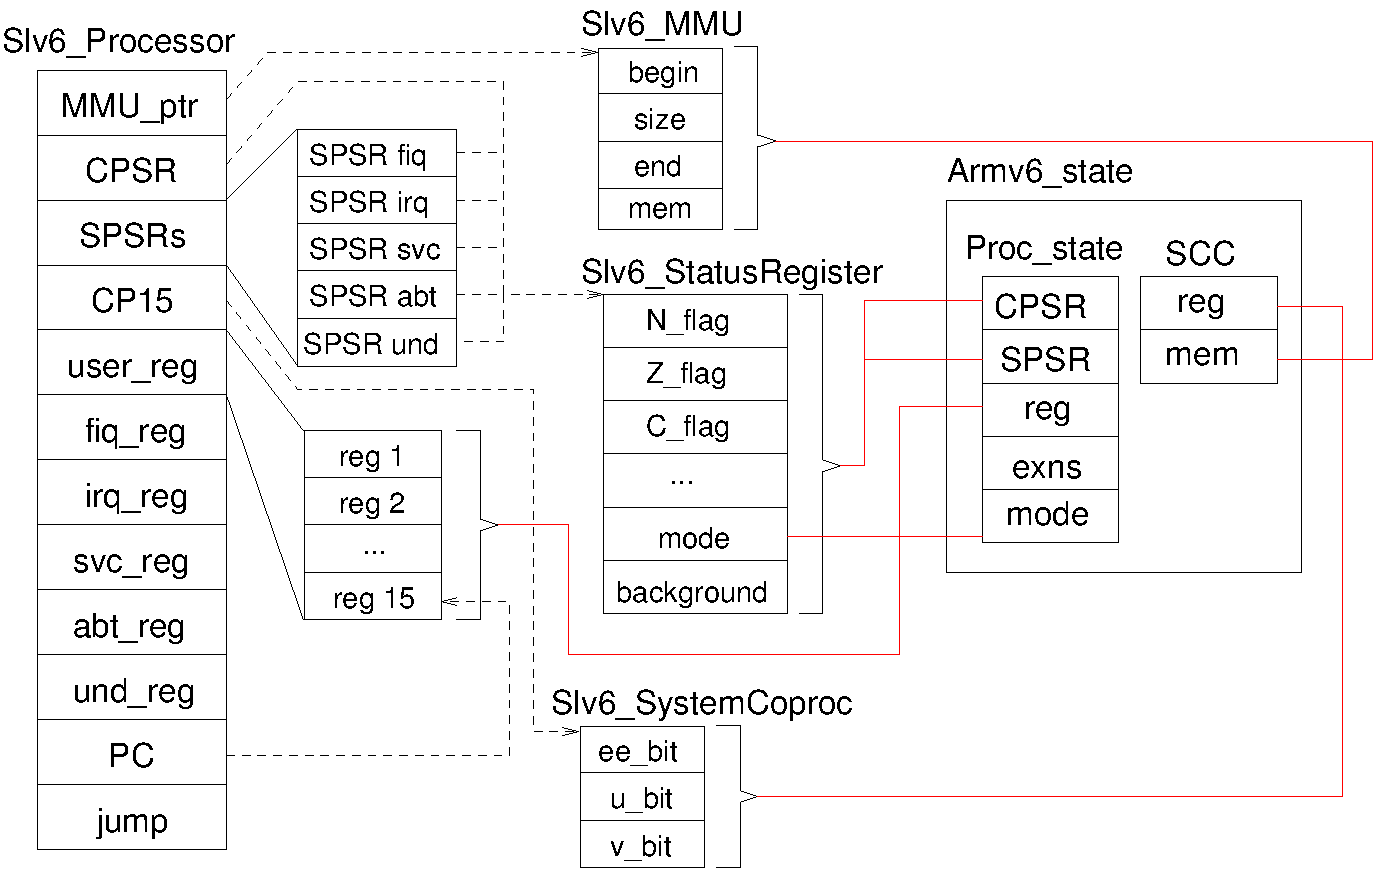
\includegraphics[width=1.01\linewidth]{fig/projection2.pdf}
\end{frame}

\begin{frame}
\frametitle{Main theorem for ADC (add with carry)}
\hfil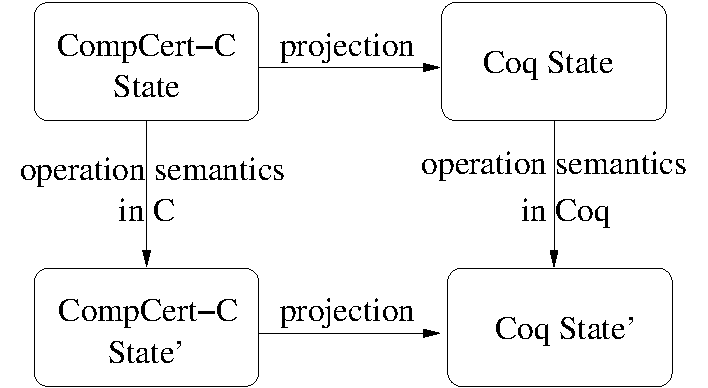
\includegraphics[width=.85\linewidth]{fig/theorem.pdf}
\end{frame}


\begin{frame}[fragile]
\frametitle{Evaluation rule of a field in CompCert C semantics}

\begin{alltt}
\small
Inductive eval_expr :
 env-> mem-> kind-> expr-> trace-> mem-> expr-> Prop:=
 ...
 | \bleu{eval_field} : \(\forall\) e m a t m' a' f ty,
    eval_expr e m RV a t m' a' ->
    eval_expr e m LV (\brique{Efield} a f ty) t m' (\violet{Efield} a' f ty)
\end{alltt}
\end{frame}

\begin{frame}[fragile]
\frametitle{Inversion function for ~\texttt{eval\_field}}
\small
\begin{alltt}
Definition \textbf{inv_field} {g} {e} {m} {ex} {t} {m'} {ex'}
  (ee:eval_expr g e m LV ex t m' ex') :=
  let \textbf{diag} e ex ex' m m' :=
    match ex with
      | \brique{Efield} a b c =>
        \(\forall\) (X:expr->Prop),
        (\(\forall\) t a', eval_expr g e m RV a t m' a' -> 
                           X (\violet{Efield} a' b c)) -> X ex'
      | _ => True
    end in
    match ee in (eval_expr _ e m _ ex _ m' ex')
             return  \textbf{diag} e ex ex' m m'  with
      | \bleu{eval_field} _ _ _ t _ a' _ _ H1 => 
          fun X k => k t a' H1
      | _ => I
    end.
\end{alltt}
\end{frame}

\begin{frame}[fragile]
\frametitle{High-level tactic for inductive type \texttt{eval\_expr}}
\begin{block}{\texttt{inv\_eval\_expr}:  ~~repeat the following steps}
\begin{itemize}
\item 
find the hypothesis we want to invert\\
(by matching the targetted memory states);
\item 
revert related hypotheses;
\item 
\bleu{call the right diagonal function;}
%(all auxiliary functions are gathered in the tactic);
\item 
\brique{give meaningful names} to derived variables and hypotheses
  (\brique{predictable} from \texttt{inv\_field}, etc.);
\item 
update all other related hypotheses;% according to the new names
%and new values;
\item 
clean up useless variables and hypotheses;
\end{itemize}
\end{block}
\end{frame}

\begin{frame}[fragile]
\frametitle{High-level tactic for inductive type \texttt{eval\_expr}}
\small
\begin{alltt}
Ltac inv_eval_expr m m' :=
  ...
  let t1_:=fresh "t" in
  let v1_:=fresh "v" in
  let ev_ex1 := fresh "ev_ex" in
  ...
  match goal with
  ...
  |[ee: eval_expr ?ge ?e m LV (\brique{Efield} ?a ?f ?ty) ?t m' ?a' 
      |- ?cl] =>
      apply (\textbf{inv_field} ee); 
      clear ee; intros t1_ a1_ ev_ex1; 
      intros;
      inv_eval_expr m m'
\end{alltt}
\end{frame}


\begin{frame}[fragile]
\frametitle{Built-in inversion}
\small
\begin{alltt}
H:eval_expr (Genv.globalenv prog_adc) e m RV
   (\brique{Ecall} (\brique{Evalof} (\brique{Evar} copy_StatusRegister T14) T14)
      (\brique{Econs}
         (\brique{Eaddrof}
            (\brique{Efield} (\brique{Ederef} (\brique{Evalof} (\brique{Evar} proc T3) T3) T6)
              adc_compcert.cpsr T7) T8)
         (\brique{Econs}
            (\brique{Ecall} (\brique{Evalof} (\brique{Evar} spsr T15) T15)
               (\brique{Econs} (\brique{Evalof} (\brique{Evar} proc T3) T3) \brique{Enil}) T8)
                \brique{Enil}))
      T12) t m' a'
============================
   proc_state_related m' e st'
\end{alltt}
\begin{alltt}
\bleu{
  inv H. inv H4. inv H9. inv H5. inv H4. inv H5. 
  inv H15. inv H4. inv H5. inv H14. inv H4. inv H3. 
  inv H15. inv H5. inv H4. inv H5. inv H21. inv H13.
  ...}
\end{alltt}
\end{frame}

\begin{frame}[fragile]
\frametitle{Handcrafted small inversion}
\small
\begin{alltt}
H:eval_expr (Genv.globalenv prog_adc) e m RV
   (\brique{Ecall} (\brique{Evalof} (\brique{Evar} copy_StatusRegister T14) T14)
      (\brique{Econs}
         (\brique{Eaddrof}
            (\brique{Efield} (\brique{Ederef} (\brique{Evalof} (\brique{Evar} proc T3) T3) T6)
              adc_compcert.cpsr T7) T8)
         (\brique{Econs}
            (\brique{Ecall} (\brique{Evalof} (\brique{Evar} spsr T15) T15)
               (\brique{Econs} (\brique{Evalof} (\brique{Evar} proc T3) T3) \brique{Enil}) T8)
                \brique{Enil}))
      T12) t m' a'
============================
   proc_state_related m' e st'
\end{alltt}
\begin{alltt}
\cvert{
  inv_eval_expr} \bleu{m m'}.
  ...


\end{alltt}
\end{frame}


\begin{frame}\frametitle{Performance}
\begin{table}[t]
\small
\centering
\caption{Time costs (in seconds)}
\label{t:timing}
\begin{tabular}{|l|c|c|c|c|}
\hline
 & \texttt{inversion} & \texttt{D. Inversion} & \texttt{BasicElim} & \texttt{hc\_inversion} \\
\hline
%Full example & 1.628102 & 0.976061 & 1.428089 & 0.31202 \\
Full ex. & 1.628 & 0.976 & 1.428 & \cvert{0.312} \\
\hline
%Ecall & 0.132009 & 0.076004 & 0.112007 &  0.028002\\
Ecall & 0.132 & 0.076 & 0.112 &  \cvert{0.028}\\
\hline
%Evalof &  0.132008 & 0.072004 & 0.092005 & 0.020001\\
Evalof &  0.132 & 0.072 & 0.092 & \cvert{0.020}\\
\hline
%Evar &  0.128008 & 0.064004 & 0.084006 & 0.024001\\
Evar &  0.128 & 0.064 & 0.084 & \cvert{0.024}\\
\hline
%Eaddrof &  0.140009 & 0.076005 & 0.104007 & 0.020001\\
Eaddrof &  0.140 & 0.076 & 0.104 & \cvert{0.020}\\
\hline
\end{tabular}
\end{table}

\begin{table}[t]
\small
\centering
\caption{Size of compilation results (in KBytes)}
\label{t:size}
\begin{tabular}{|l|c|c|c|c|}
\hline
 & \texttt{inversion} & \texttt{D. Inversion} & \texttt{BasicElim} & \texttt{hc\_inversion} \\
\hline
%Full example & 191346 & 459613 & 170821 & 36712\\
Full ex. & 191 & 460 & 171 & \cvert{37}\\
\hline
\end{tabular}
\end{table}
\small
   D. Inversion = Derived Inversion
\end{frame}


\begin{frame}
\frametitle{Conclusion}

%Small inversions are beautiful

\Large

\begin{centering}

Yes you can 

\bigskip

do inversions by yourself

\end{centering}

\end{frame}


\begin{frame}

\Huge

\hfil Thanks!

\vfill
%\bigskip

\hfil Questions?

\end{frame}


\end{document}

%%% Local Variables: 
%%% mode: latex
%%% TeX-master: "oral-itp13"
%%% End: 
